\chapter{Evaluation}
\label{chap:eval}



This section reports the evaluation results of the NeSC prototype.
We examine the performance benefits of enabling VMs to directly access NeSC, and compare its performance to those of virtio and device emulation.
%% , and raw access to the device by the hypervisor without the virtualization layer.
Our baseline storage device is the NeSC PF, which presents the hypervisor a raw storage device with no file mapping capabilities. The baseline measurement is done by the hypervisor without any virtualization layer.

%%%%%%%%%%%%%%%%%%%%%%%%%%%%%%%%%%%%%%%%%%%%%%%%%%
\section*{Raw device performance}
%%%%%%%%%%%%%%%%%%%%%%%%%%%%%%%%%%%%%%%%%%%%%%%%%%

We begin by examining the raw device performance observed by the guest VM when accessing a virtual NeSC device. A file on the hypervisor's filesystem is used to create a VF, which is then mapped to the guest VM. These results are compared to mapping the PF itself to the guest VM using either virtio and device emulation. The baseline (marked \emph{Host} in the figures) is the performance observed when the hypervisor directly accesses the PF block device (without virtualization).
In all configurations, we examine the performance of reads and writes to the raw virtual device, without creating a filesystem. 

When a guest accesses the device using virtio or device emulation, each access  request is processed by the guest I/O stack and storage device driver, delivered to the hypervisor, and is then processed by the hypervisor's I/O stack and its own device driver.
When directly assigning a NeSC VF to the guest, requests pass down the guest I/O stack directly to the device. In contrast, in the baseline evaluation (i.e., \emph{Host} in the figure) the requests only pass down the hypervisor I/O stack.

The performance itself was measured using \emph{dd}~\cite{coreutils} for different block sizes.

%%%%%%%%%%%%%%%%%%%%
\begin{figure}[t]
  \centering
  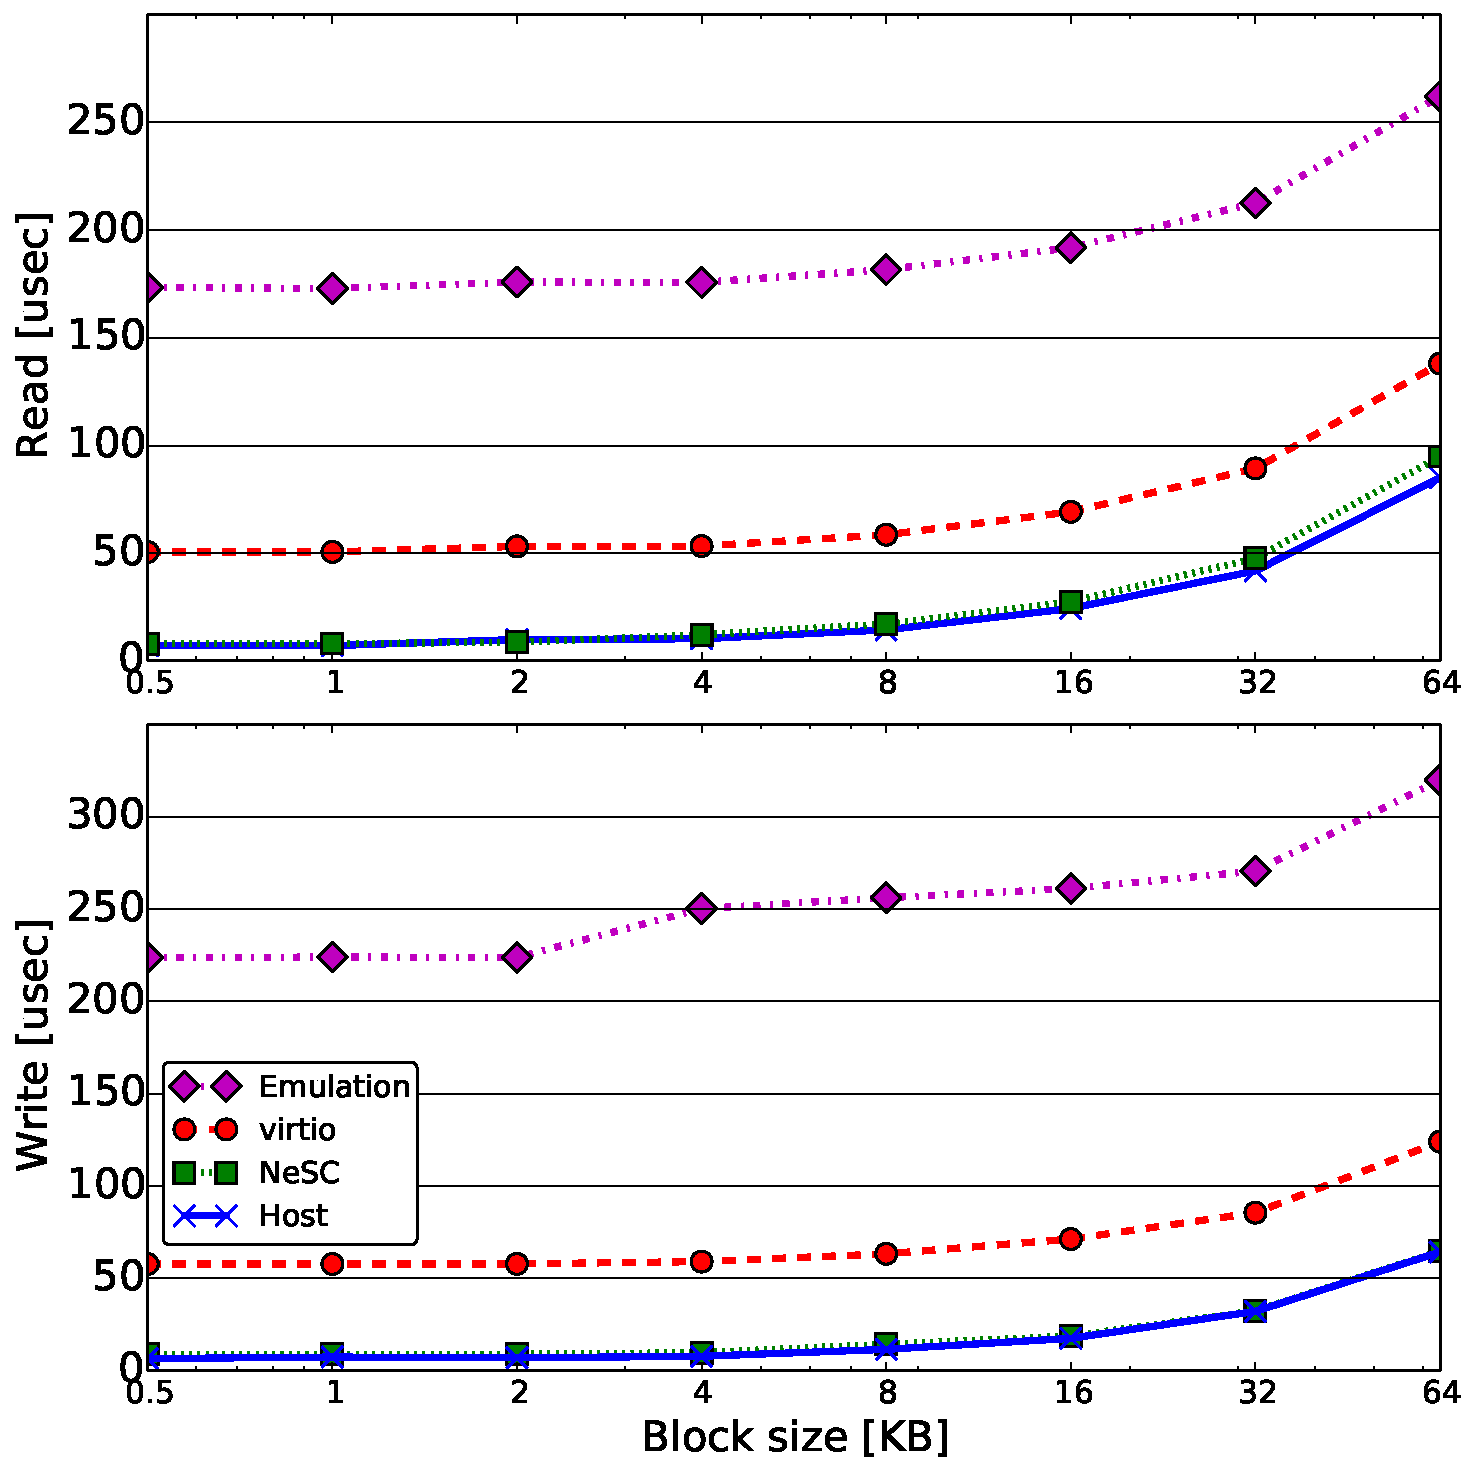
\includegraphics[width=1\columnwidth]{figs/latency_block_size.pdf}
  \caption{Raw access latency observed for read (top) and write (bottom) operations for different block sizes.}
  \label{fig:latency}
\end{figure}
%%%%%%%%%%%%%%%%%%%%

\section*{NeSC latency}
Figure~\ref{fig:latency} shows the latency observed for read (top) and write (bottom) operations, using request sizes varying from 512B to 32KB. The figure shows that the latency obtained by NeSC for both read and write is similar to that obtained by the host when directly accessing the PF. Furthermore, the NeSC latency is  over \speedup{6} faster than virtio and over \speedup{20} faster than device emulation for accesses smaller than 4KB.

%%%%%%%%%%%%%%%%%%%%
\begin{figure}[t]
  \centering
  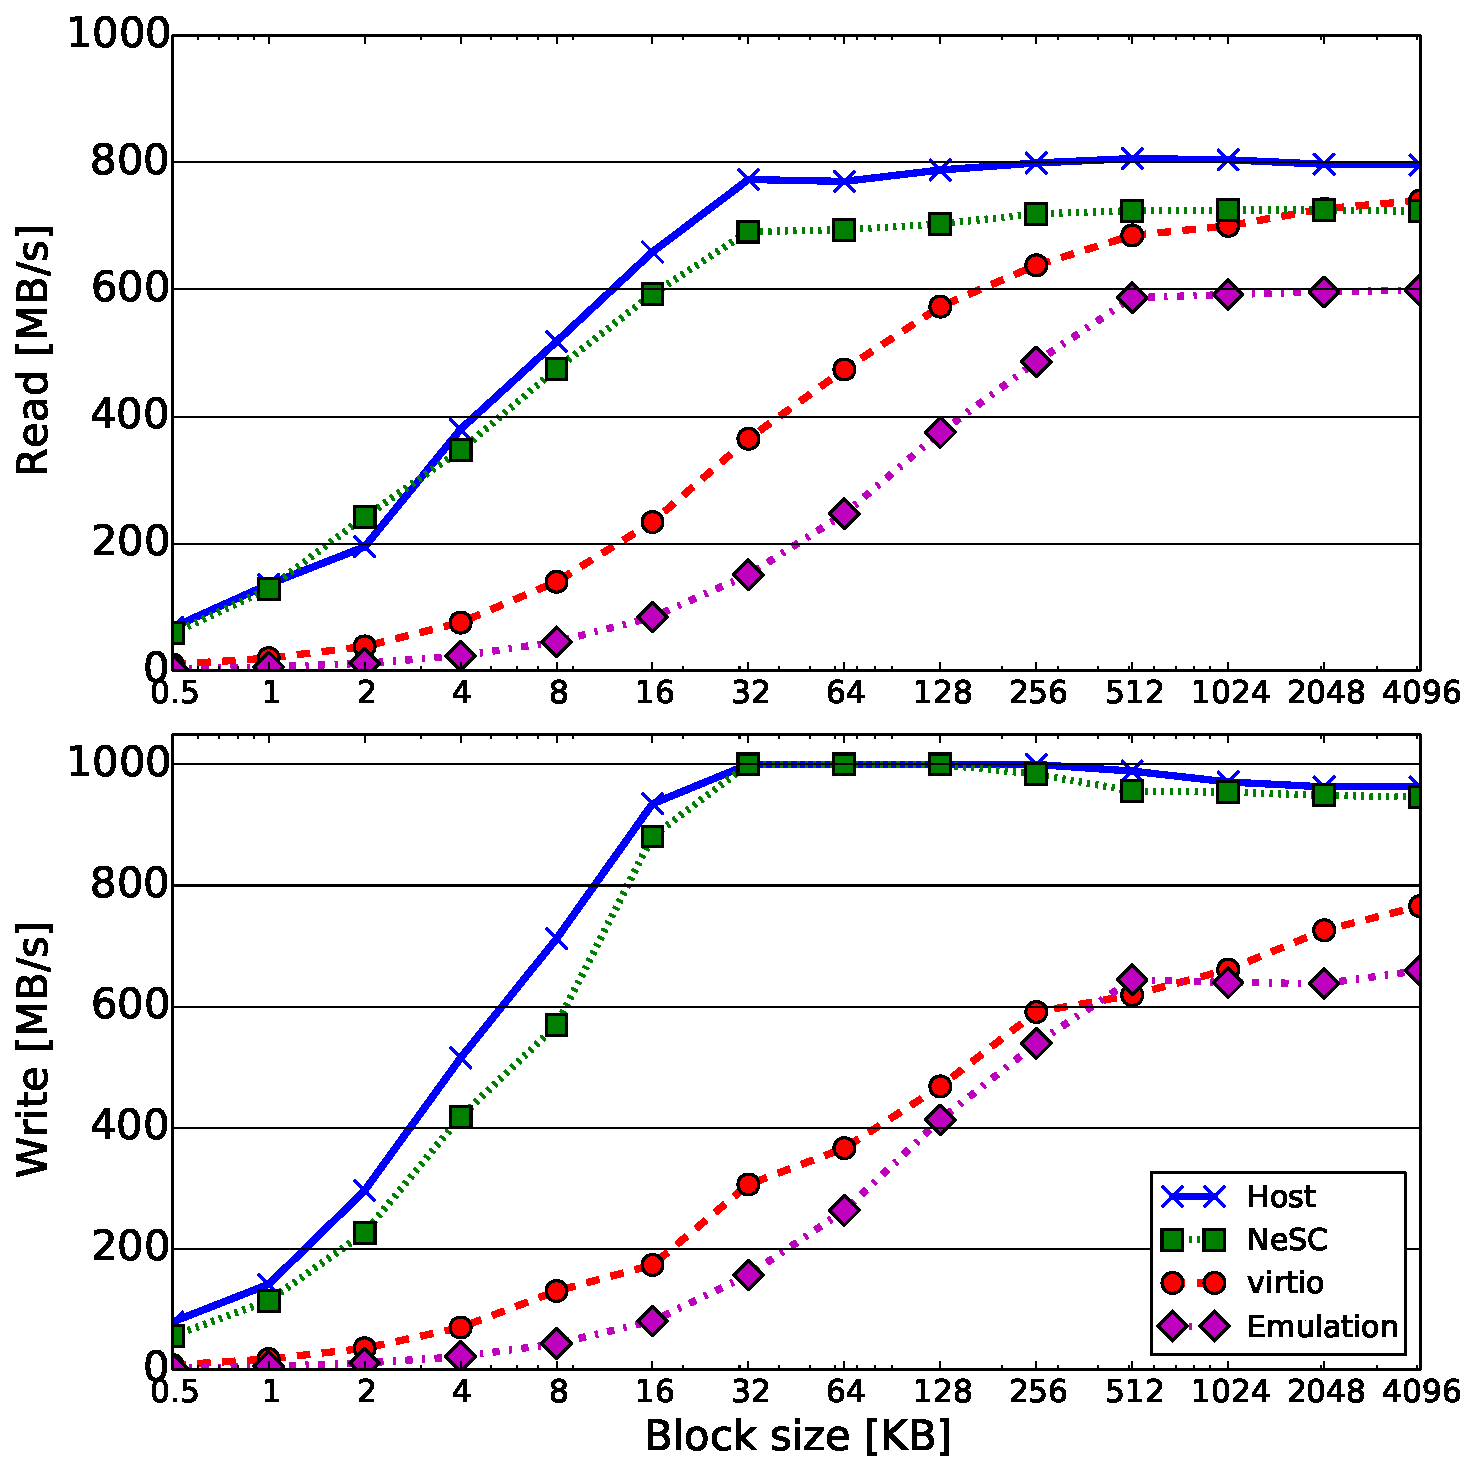
\includegraphics[width=1\columnwidth]{figs/throughput_block_size.pdf}
  \caption{Raw bandwidth observed for read (top) and write (bottom) operations for different block sizes.}
  \label{fig:bw}
\end{figure}
%%%%%%%%%%%%%%%%%%%%

\section*{NeSC bandwidth}
Figure~\ref{fig:bw} shows the bandwidth delivered for read (top) and write (bottom) operations, using request sizes varying from 512B to 32KB.

We begin by examining the read bandwidth.
%
The figure shows that for reads smaller than 16KB, NeSC obtained bandwidth close to that of the baseline and outperforms virtio by over \speedup{2.5}.
%
Furthermore, for very large block sizes (over 2MB), the bandwidths delivered by NeSC and virtio converge. This is because such large accesses ameliorate the overheads incurred by VM/hypervisor traps (vmenter/vmexit on Intel platforms).

When examining the write bandwidth, we observe that NeSC delivers performance similar to the baseline for all block sizes. This result is better than that achieved for read bandwidth, for which NeSC is \tilde\percent{10} slower than  the baseline for blocks of size 32KB and larger. Moreover, NeSC's write bandwidth is consistently and substantially better than virtio and emulation, peaking at over \speedup{3} for 32KB block sizes.


%%%%%%%%%%%%%%%%%%%%
\begin{figure}[t]
  \centering
  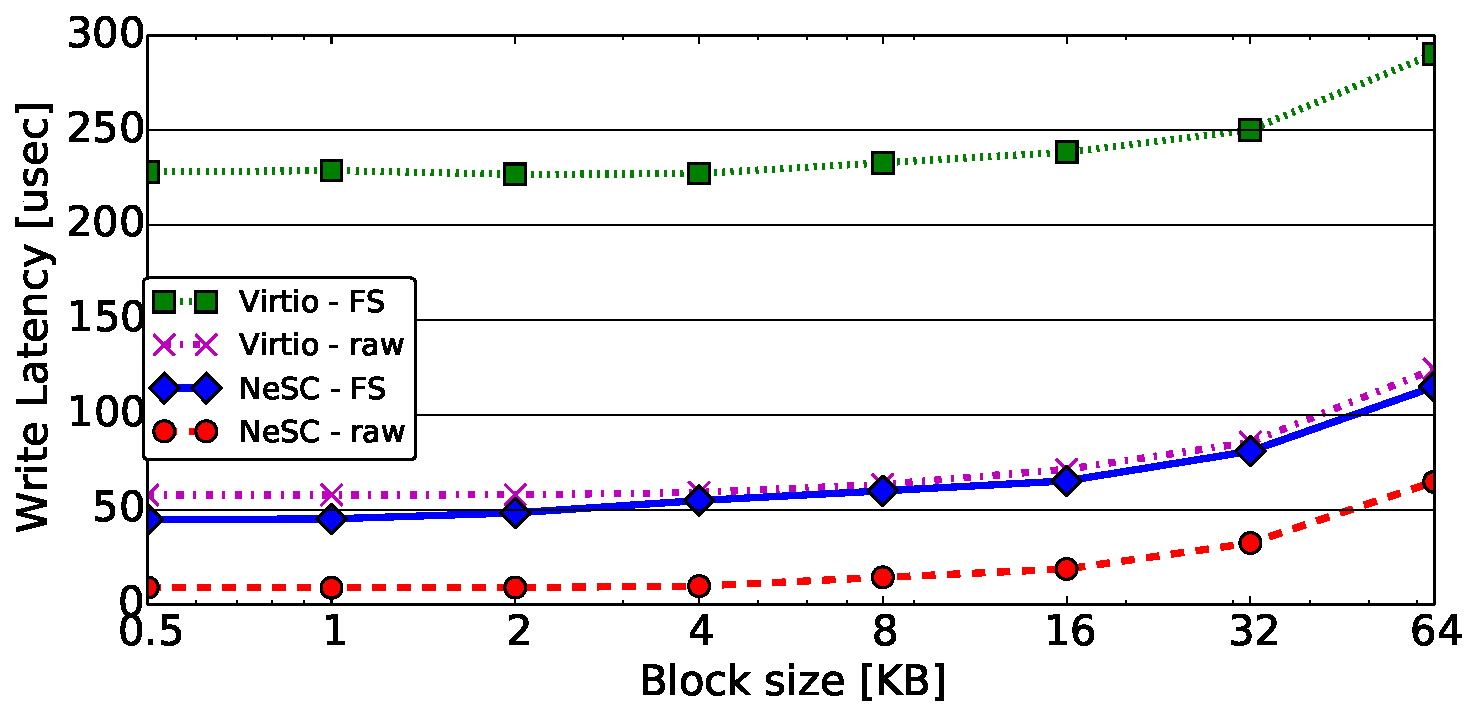
\includegraphics[width=1\columnwidth]{figs/fs_affect.pdf}
  \caption{Filesystem overheads.}
  \label{fig:fs_effect}
\end{figure}
%%%%%%%%%%%%%%%%%%%%

\section*{Filesystem overheads}
We next examine the overheads incurred by filesystem translations. To this end, we compare the access latency observed by the guest VM when accessing the raw device with that observed when accessing an ext4 filesystem on the virtual device.

Figure~\ref{fig:fs_effect} shows the write latency when accessing the device with and without a filesystem, for NeSC and virtio virtualization (for brevity, we omit the results obtained using an emulated device since they were much worse than virtio). We only show results for writes because those are more prohibitive for NeSC, since writes may require the VF to request extent allocations from the OS's filesystem.

The figure demonstrates the performance benefits of NeSC. While the filesystem overhead consistently increases NeSC's write latency by \tilde 40\us, the latency obtained using NeSC is similar to that of a raw virtio device. Using virtio with a filesystem incurs an extra \tilde 170\us, which is over \speedup{4} slower than NeSC with a filesystem for writes smaller than 8KB.

We note that the similar latencies observed when using a filesystem with NeSC and when using a raw virtio device indicate that NeSC effectively eliminates the hypervisor's filesystem overheads.

%%%%%%%%%%%%%%%%%%%%%%%%%%%%%%%%%%%%%%%%%%%%%%%%%%
\section*{Application performance}
%%%%%%%%%%%%%%%%%%%%%%%%%%%%%%%%%%%%%%%%%%%%%%%%%%

%%%%%%%%%%%%%%%%%%%%
\begin{figure}[t]

  %% \vspace*{-1.5ex}
  \centering
  \subfloat[Applications speedups when using NeSC over device emulation.]{
    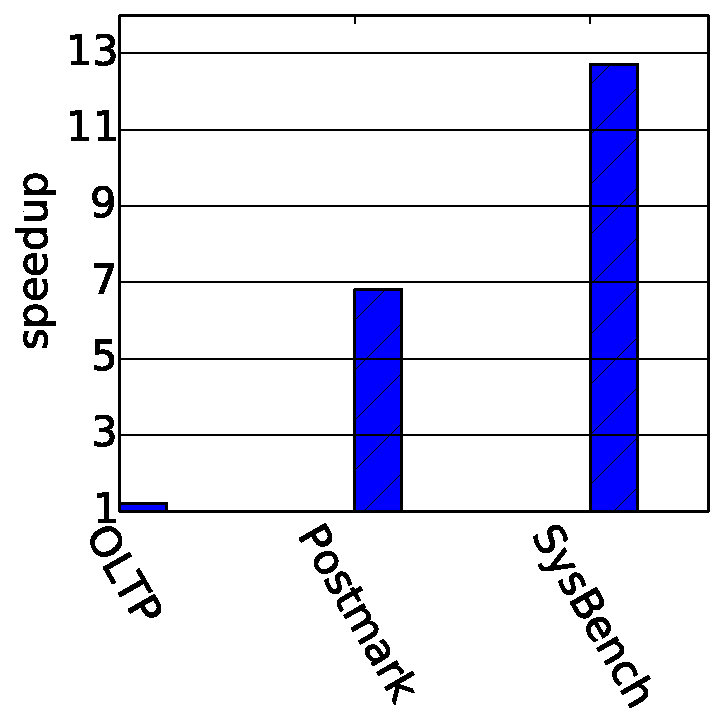
\includegraphics[width=0.48\columnwidth]{figs/application_benchmark_emulation.pdf}
 %   \caption{Read Flow}
    \label{fig:apps_emulation}
  }
  %
  \subfloat[Application speedups when using NeSC over virtio.]{
    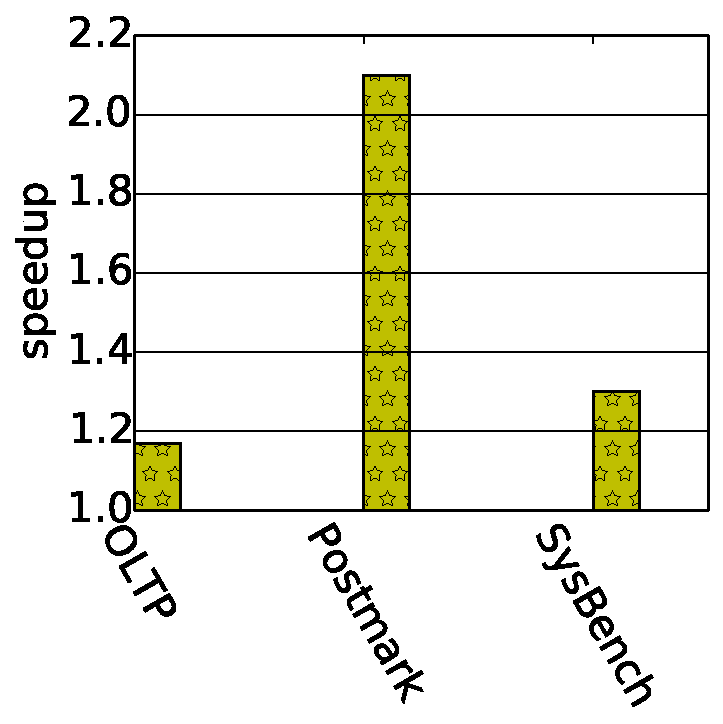
\includegraphics[width=0.48\columnwidth]{figs/application_benchmark_virtio.pdf}
    \label{fig:apps_virtio}
  }
  \caption{Application speedups over other storage virtualization methods.\label{fig:apps}}

    
\end{figure}
%%%%%%%%%%%%%%%%%%%%

We finally examine how the raw performance delivered by NeSC translates to application level speedups. To this end, we compare the performance of the  applications (listed in Figure~\ref{tab:bench}) when running in a guest Linux VM whose storage device is mapped to a NeSC VF, to a virtio device and to a fully emulated device.

The virtual storage device is mapped to the VM in the following manner. The hypervisor creates an ext4 filesystem on the raw device using the NeSC PF. The virtual storage device is stored as an image file (with ext4 filesystem) on  the hypervisor's filesystem, and the hypervisor maps the file to the VM using either of the mapping facilities: virtio, emulation or a NeSC VF.

Figure~\ref{fig:apps} shows the application speedups obtained using a NeSC VF device over device emulation and virtio. For the MySQL OLTP benchmark, the figure shows that mapping the virtual disk using a NeSC virtual device improves performance by \speedup{1.2} over both device emulation (Figure~\ref{fig:apps_emulation}) and virtio (Figure~\ref{fig:apps_virtio}).

The performance improvements provided by NeSC are even more substantial for Postmark and Sysbench File I/O.
Postmark enjoys more than \speedup{6} speedup over device emulation and more than \speedup{2} over virtio. Sysbench File I/O, on the other hand, enjoys a dramatic \speedup{13} speedup over device emulation, and \speedup{1.3} over virtio.

In summary, the evaluation of the NeSC prototype demonstrates its substantial performance benefits over state-of-the-art storage virtualization methods. The benefits are consistent for both read and write microbenchmarks and for common storage benchmarks.

